
\begin{figure}[!b]
	\centering

	% -0,00D (lens) compared with: -0,00D, -1,00D, -2,00D, -3,00D and -4,00D (simulated)
	\subfigure[]{
		
\includegraphics[width=0.17\linewidth]{__Images/05/group5_f5.0/similarity/bw_N_20-200__-0,00D_compared_with-0,00D.png}
	}
	~
	\subfigure[]{
		
\includegraphics[width=0.17\linewidth]{__Images/05/group5_f5.0/similarity/bw_N_20-200__-0,00D_compared_with-1,00D.png}
	}
	~
	\subfigure[]{
		
\includegraphics[width=0.17\linewidth]{__Images/05/group5_f5.0/similarity/bw_N_20-200__-0,00D_compared_with-2,00D.png}
	}
	~
	\subfigure[]{
		
\includegraphics[width=0.17\linewidth]{__Images/05/group5_f5.0/similarity/bw_N_20-200__-0,00D_compared_with-3,00D.png}
	}
	~
	\subfigure[]{
		
\includegraphics[width=0.17\linewidth]{__Images/05/group5_f5.0/similarity/bw_N_20-200__-0,00D_compared_with-4,00D.png}
	}
	% -1,00D (lens) compared with: -0,00D, -1,00D, -2,00D, -3,00D and -4,00D (simulated)
	\subfigure[]{
		
\includegraphics[width=0.17\linewidth]{__Images/05/group5_f5.0/similarity/bw_N_20-200__-1,00D_compared_with-0,00D.png}
	}
	~
	\subfigure[]{
		
\includegraphics[width=0.17\linewidth]{__Images/05/group5_f5.0/similarity/bw_N_20-200__-1,00D_compared_with-1,00D.png}
	}
	~
	\subfigure[]{
		
\includegraphics[width=0.17\linewidth]{__Images/05/group5_f5.0/similarity/bw_N_20-200__-1,00D_compared_with-2,00D.png}
	}
	~
	\subfigure[]{
		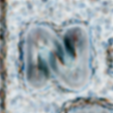
\includegraphics[width=0.17\linewidth]{__Images/05/group5_f5.0/similarity/bw_N_20-200__-1,00D_compared_with-3,00D.png}
	}
	~
	\subfigure[]{
		
\includegraphics[width=0.17\linewidth]{__Images/05/group5_f5.0/similarity/bw_N_20-200__-1,00D_compared_with-4,00D.png}
	}
	% -2,00D (lens) compared with: -0,00D, -1,00D, -2,00D, -3,00D and -4,00D (simulated)
	\subfigure[]{
		
\includegraphics[width=0.17\linewidth]{__Images/05/group5_f5.0/similarity/bw_N_20-200__-2,00D_compared_with-0,00D.png}
	}
	~
	\subfigure[]{
		
\includegraphics[width=0.17\linewidth]{__Images/05/group5_f5.0/similarity/bw_N_20-200__-2,00D_compared_with-1,00D.png}
	}
	~
	\subfigure[]{
		
\includegraphics[width=0.17\linewidth]{__Images/05/group5_f5.0/similarity/bw_N_20-200__-2,00D_compared_with-2,00D.png}
	}
	~
	\subfigure[]{
		
\includegraphics[width=0.17\linewidth]{__Images/05/group5_f5.0/similarity/bw_N_20-200__-2,00D_compared_with-3,00D.png}
	}
	~
	\subfigure[]{
		
\includegraphics[width=0.17\linewidth]{__Images/05/group5_f5.0/similarity/bw_N_20-200__-2,00D_compared_with-4,00D.png}
	}
	% -3,00D (lens) compared with: -0,00D, -1,00D, -2,00D, -3,00D and -4,00D (simulated)
	\subfigure[]{
		
\includegraphics[width=0.17\linewidth]{__Images/05/group5_f5.0/similarity/bw_N_20-200__-3,00D_compared_with-0,00D.png}
	}
	~
	\subfigure[]{
		
\includegraphics[width=0.17\linewidth]{__Images/05/group5_f5.0/similarity/bw_N_20-200__-3,00D_compared_with-1,00D.png}
	}
	~
	\subfigure[]{
		
\includegraphics[width=0.17\linewidth]{__Images/05/group5_f5.0/similarity/bw_N_20-200__-3,00D_compared_with-2,00D.png}
	}
	~
	\subfigure[]{
		
\includegraphics[width=0.17\linewidth]{__Images/05/group5_f5.0/similarity/bw_N_20-200__-3,00D_compared_with-3,00D.png}
	}
	~
	\subfigure[]{
		
\includegraphics[width=0.17\linewidth]{__Images/05/group5_f5.0/similarity/bw_N_20-200__-3,00D_compared_with-4,00D.png}
	}
	% -4,00D (lens) compared with: -0,00D, -1,00D, -2,00D, -3,00D and -4,00D (simulated)
	\subfigure[]{
		
\includegraphics[width=0.17\linewidth]{__Images/05/group5_f5.0/similarity/bw_N_20-200__-4,00D_compared_with-0,00D.png}
	}
	~
	\subfigure[]{
		
\includegraphics[width=0.17\linewidth]{__Images/05/group5_f5.0/similarity/bw_N_20-200__-4,00D_compared_with-1,00D.png}
	}
	~
	\subfigure[]{
		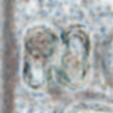
\includegraphics[width=0.17\linewidth]{__Images/05/group5_f5.0/similarity/bw_N_20-200__-4,00D_compared_with-2,00D.png}
	}
	~
	\subfigure[]{
		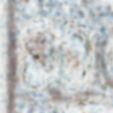
\includegraphics[width=0.17\linewidth]{__Images/05/group5_f5.0/similarity/bw_N_20-200__-4,00D_compared_with-3,00D.png}
	}
	~
	\subfigure[]{
		
\includegraphics[width=0.17\linewidth]{__Images/05/group5_f5.0/similarity/bw_N_20-200__-4,00D_compared_with-4,00D.png}
	}	
	
	\caption[Visualization of the local structural similarity index of the hyperopic results]{Visualization of the local structural similarity index when comparing the hyperopic results. For each image captured by a DSLR camera (Figures~\ref{fig:blur_progression_neg}(a-e)) we compare it to the ones generated with our method (Figures~\ref{fig:blur_progression_neg}(f-j)). The first row shows the local SSIM index when comparing the image captured with no additional lenses to -0D simulation (a); -1D simulation (b); -2D simulation (c); -3D simulation (d); and -4D simulation (e). The others follow the same ideia, however, varying the diopter of the additional lens.}
	\label{fig:bw_similarity}
\end{figure}